\documentclass[oneside,12pt,openright]{report} % IL setup attuale è doppia faccia

\usepackage[utf8]{inputenc}
\usepackage[italian]{babel} %Se si vuole utilizzare l'italiano cambiare "english" in "italian"
\usepackage[a4paper,top=3cm,bottom=3cm,left=3cm,right=3cm,marginparwidth=1.5cm,bindingoffset=15mm,heightrounded]{geometry}
\usepackage{csquotes}
\usepackage{quoting}
\quotingsetup{font=small}

% Times new Roman font e interlinea a 1.5 (mandatorie Mercatorum)
\usepackage{times}
\linespread{1.5}

% Per creare box colorati
\usepackage{tcolorbox}

\usepackage{mdframed}

% Definiamo uno stile per la vignetta
\tcbset{
    myvignette/.style={
        colback=gray!20,   % Sfondo grigio chiaro
        colframe=black,     % Bordo nero
        coltitle=white,     % Titolo bianco
        fonttitle=\bfseries,% Titolo in grassetto
        boxrule=1pt,        % Spessore del bordo
        rounded corners,    % Angoli arrotondati
        width=\textwidth,   % Larghezza pari alla pagina
        sharp corners=north,% Angolo superiore non arrotondato
        title={Caso Particolare} % Titolo di default
    }
}

\usepackage{amssymb}
\usepackage{amsmath}
\usepackage{graphicx}
% ------------------------------------------------------------------------------------------Format generale per inserire immagini
%\begin{figure}[htbp]
    %\centering
    %\includegraphics[width=0.7\textwidth]{nome_file_immagine}
    %\caption{Descrizione dell'immagine}
    %\label{fig:etichetta_per_riferimento}
%\end{figure}
%-------------------------------------------------------------------------------------------

\usepackage[colorlinks=true, allcolors=black]{hyperref} % Si può modificare allcolors=blue per una migliore visione in fase di produzione

% Per inserire codice MATLAB
\usepackage{xcolor}% Per la colorazione del codice
\usepackage{colortbl}
\usepackage{array}
\usepackage{listings}


\lstdefinestyle{MatlabStyle}{% Se si usa un altro linguaggio, modificare "language"
    language=Matlab,
    basicstyle=\ttfamily\footnotesize,
    keywordstyle=\color{blue},
    commentstyle=\color{green!50!black},
    stringstyle=\color{red},
    backgroundcolor=\color{gray!10},
    frame=single,
    rulecolor=\color{black},
    breaklines=true,
    numbers=left,
    numberstyle=\tiny,
    stepnumber=1,
    numbersep=5pt
}

\lstdefinestyle{LogStyle}{
    basicstyle=\ttfamily\small,
    breaklines=true,                % Fondamentale per non uscire dai margini
    backgroundcolor=\color{gray!10},
    frame=single,
    rulecolor=\color{gray!30},
    xleftmargin=10pt,
    showstringspaces=false
}
% ---------------------------------------------------------------------------------------------Da usare per fare il matlab style \begin{lstlisting}[style=MatlabStyle, caption={}, label={lst:}] ------------------------------------------------------------------------------------------------------


\usepackage{booktabs}

\usepackage{tikz}

% TikZ libraries
\usetikzlibrary{positioning, arrows.meta, shapes.geometric}

% TikZ styles
\tikzstyle{vertex}=[circle, draw, thick, minimum size=15pt, inner sep=1pt]
\tikzstyle{edge label}=[midway, fill=white, inner sep=1pt, font=\footnotesize]
\tikzstyle{directed edge}=[-{Latex[length=2mm]}, thick]
\tikzstyle{undirected edge}=[thick]

\usepackage{algorithm}% For algorithm environment
\usepackage{algpseudocode} % For pseudocode layout
% Define argmin operator if not available
\DeclareMathOperator*{\argmin}{arg\,min}

\usepackage[style=apa, backend=biber]{biblatex}
\addbibresource{references.bib} % OK
\usepackage{lipsum}


% Minted da noie, quindi usiamo sto coso:
\usepackage{listings}
\usepackage{xcolor}


% Definizione colori stile "VsCode Light"
\definecolor{keywordcolor}{rgb}{0.0, 0.0, 1.0}   % Blu
\definecolor{stringcolor}{rgb}{0.6, 0.1, 0.1}    % Rosso scuro
\definecolor{commentcolor}{rgb}{0.0, 0.5, 0.0}   % Verde
\definecolor{numbercolor}{rgb}{0.5, 0.5, 0.5}    % Grigio
\definecolor{backgroundcolor}{rgb}{0.97, 0.97, 0.97} % Grigio chiarissimo

\lstset{
    backgroundcolor=\color{backgroundcolor},
    basicstyle=\ttfamily\small,
    breakatwhitespace=false,
    breaklines=true,
    captionpos=b,
    commentstyle=\color{commentcolor},
    keepspaces=true,
    keywordstyle=\color{keywordcolor},
    numbers=left,
    numbersep=10pt,
    numberstyle=\tiny\color{numbercolor},
    rulecolor=\color{black!30},
    showspaces=false,
    showstringspaces=false,
    showtabs=false,
    stepnumber=1,
    stringstyle=\color{stringcolor},
    tabsize=2,
    frame=lines % Linea sopra e sotto il codice
}

% Setup specifico per JSON
\lstdefinelanguage{json}{
    morestring=[b]",
    morestring=[d]'
}

\usepackage{tabularx}

\begin{document}

\newgeometry{top=3cm,bottom=3cm,left=3cm,right=3cm,heightrounded}
\begin{titlepage}
    \begin{figure}[!htb]
        \centering
        
\includegraphics[keepaspectratio=true,scale=3.5]{Immagini/Mercatorum logo.jpg} % Placeholder
        %\rule{5cm}{3cm} % Placeholder for the image
    \end{figure}

    \begin{center}
        \vspace{5mm}
        \large{\textbf{FACOLTÀ DI SCIENZE TECNOLOGICHE E DELL'INNOVAZIONE}}
        \vspace{1.5mm}

        \noindent\rule{225pt}{0.4pt}

        \vspace{5mm}

        \large{\textbf{CORSO DI LAUREA IN INGEGNERIA INFORMATICA}}

        \vspace{10mm}

        \Large{\textbf{\emph{Prova Finale in}}}

        \large{\textbf{PROGRAMMAZIONE}}

        \vspace{1mm}

        \large{Dall'analisi dei log HTTP al rilevamento automatico di anomalie, un approccio basato su Machine Learning}

    \end{center}

    \vspace{15mm}

    \begin{minipage}[t]{0.33\textwidth} % Relatore minipage (kept for context)
        \centering % Center the content within this minipage
        {\large RELATORE\\[0.5em]
            \normalsize Chiar.mo\\ % Removed centering here, as \centering above handles it
            Mauro Bellone}
    \end{minipage}
    \hfill % Pushes the minipages apart
    \begin{minipage}[t]{0.35\textwidth} % <-- REMOVED \raggedleft
        \centering % <--- ADDED \centering switch here
        {\large CANDIDATO\\[0.5em] % Braces keep \large local
            \large FEDERICO MANINI\\[0.5em]
            \normalsize MATR.0082200317 } % Braces keep \normalsize local
    \end{minipage}

    \vspace{20mm}

    \centering{\normalsize{Anno Accademico 2022/2025}}

\end{titlepage}
\restoregeometry


\newpage
\null
\newpage


\vspace{30cm}


\begin{flushright}
    \emph{A papà\dots}

    \emph{\dots Chi sa, sa}
\end{flushright}

\tableofcontents

\chapter*{Introduzione}
\addcontentsline{toc}{chapter}{Introduzione}

\section*{Obiettivi}
\addcontentsline{toc}{section}{Obiettivi}

Negli ultimi anni il traffico web ha assunto un ruolo centrale nell’infrastruttura digitale globale. Applicazioni distribuite, servizi \emph{cloud}, piattaforme \emph{e-commerce }e sistemi informativi aziendali si basano su architetture \emph{client–server} che utilizzano il protocollo \emph{HTTP} (\emph{Hyper-Text Transfer Protocol}) come meccanismo primario di comunicazione. In tale contesto, i server web producono una quantità significativa di dati sotto forma di \emph{log}, che rappresentano una fonte informativa preziosa per finalità di monitoraggio, sicurezza, \emph{debugging} e analisi comportamentale.

Parallelamente, l’aumento della superficie di esposizione dei servizi \emph{web} ha reso sempre più rilevante l’individuazione tempestiva di comportamenti anomali, accessi sospetti e pattern di traffico non conformi al normale utilizzo dell’applicazione. Tecniche tradizionali basate su regole statiche o \emph{blacklist} manuali mostrano limiti in termini di scalabilità e adattabilità a contesti dinamici. In questo scenario, l’applicazione di metodologie di analisi automatizzata e di tecniche di \emph{machine learning} rappresenta un approccio promettente per l’identificazione di anomalie nei log dei server web.

La presente tesi si colloca all’intersezione tra programmazione, analisi dei dati e sistemi web, con l’obiettivo di progettare e implementare un sistema prototipale per l’analisi automatica dei \emph{log HTTP} e l’individuazione di comportamenti anomali.

L’elaborato non si limita a una trattazione teorica, ma prevede la realizzazione di un caso di studio concreto basato sulla generazione e raccolta di log reali provenienti da un’applicazione web sviluppata e distribuita.

\section*{Metodologia}
\addcontentsline{toc}{section}{Metodologia}
Il caso di studio presentato in questo elaborato si basa sull’analisi di un dataset di \emph{log HTTP} già esistente, opportunamente selezionato e sottoposto a un processo di anonimizzazione e censura dei dati sensibili. In particolare, sono stati rimossi o mascherati elementi quali indirizzi IP completi, eventuali identificativi personali e informazioni riconducibili a utenti specifici, nel rispetto dei principi di minimizzazione e protezione dei dati.

Il dataset utilizzato contiene richieste \emph{HTTP} provenienti da un’applicazione web reale e comprende sia traffico ordinario sia richieste anomale o potenzialmente malevole inserite artificialmente. Prima dell’analisi, i log sono stati sottoposti a una fase di \emph{pre-processing}, comprendente \emph{parsing} strutturato, normalizzazione dei campi rilevanti e trasformazione in un formato idoneo all’elaborazione tramite algoritmi di \emph{machine learning}.

\chapter{Struttura di un log HTTP e Machine Learning}
\section{Il protocollo HTTP in generale }
In telecomunicazioni ed informatica \emph{l’HyperText Transfer Protocol} è un protocollo di tipo applicativo usato come principale sistema per la trasmissione di informazioni su internet. La prima versione del protocollo, la HTTP/0.9, venne implementata da Tim Berners-Lee, allora studioso del CERN di Ginevra ed aveva come fine ultimo la condivisione di informazioni tra la comunità scientifica \parencite{berners1989}

Successivamente vennero rilasciate versioni che rispondevano, man mano, alle esigenze che si manifestavano.

In breve:
\begin{itemize}
    \item HTTP/1.0, la prima versione effettivamente disponibile del protocollo ed implementata dallo stesso Berners-Lee \parencite{rfc1945}
    \item HTTP/1.1, presentato come RFC 2068 \parencite{rfc2068} ed aggiornato come descritto nel RFC 2616 \parencite{rfc2616}
    \item HTTP/2 e HTTP/3 pubblicate rispettivamente nelle RFC 7540 \parencite{rfc7540}  e RFC 9114 \parencite{rfc9114}
\end{itemize}

Il protocollo HTTP, come definito nell’RFC9110, lavora al livello più alto dello standard OSI \parencite{rfc9110}  con un tipo di architettura definito client/server dove il client esegue una richiesta ed il server restituisce la risposta mandata da un altro host. Nell’uso quotidiano il client corrisponde al browser mentre il server (sia quest’ultimo virtuale o fisico) è la macchina su cui risiede il sito web.

\section{Log HTTP, definizione e struttura }
Pur non esistendo una definizione formale di \emph{log HTTP} all’interno delle specifiche del protocollo, con tale espressione si fa riferimento al file generato dal server web che registra in maniera strutturata le richieste ricevute e le relative risposte fornite. Il log rappresenta dunque una traccia persistente dell’attività del server e costituisce uno strumento fondamentale per il monitoraggio della sicurezza, la diagnosi di errori applicativi, l’analisi delle performance e lo studio del traffico.

Il primo formato strutturato per i log web è il Common Log Format (CLF), sviluppato nell’ambito del progetto NCSA HTTPd \parencite{w3clogging}, presso il National Center for Supercomputing Applications. Si riporta di seguito estratto dell’archivio del World Wide Web Consortium che descrive la struttura del CLF (si veda la figura \ref{fig:clf}).

\begin{figure}[H]
    \centering
    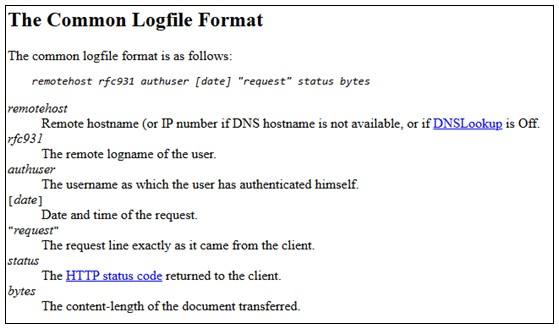
\includegraphics[width=\textwidth]{Immagini/CLF.jpg}
    \caption{W3C - Common Logfile Format}
    \label{fig:clf}
\end{figure}

Un esempio concreto risulta così strutturato:

\begin{lstlisting}[style=LogStyle]
127.0.0.1 - frank [10/Oct/2000:13:55:36 -0700] "GET /index.html HTTP/1.0" 200 2326
\end{lstlisting}

Ogni riga risulta essere una singola richiesta HTTP e contiene informazioni relative al client, al tipo di richiesta al codice di stato restituito ed infine la dimensione della risposta.

\section{Log HTTP, Datamodel per il caso studio}

Per il caso di studio oggetto della presente tesi, ci si avvale di un dataset precostruito e pubblicamente disponibile, scaricato dalla piattaforma Zenodo \parencite{zenodoLog} , repository open-access per la condivisione di dati di ricerca.

Il dataset selezionato contiene log HTTP provenienti da un ambiente reale e già sottoposti a un processo di anonimizzazione, al fine di garantire la tutela di eventuali informazioni sensibili. Tale scelta consente di operare su dati realistici, mantenendo al contempo conformità ai principi di protezione dei dati.

Di seguito si riporta un estratto esemplificativo di una riga di log convertito in formato JSON tratta dal dataset:

\begin{lstlisting}[style=LogStyle]
{
    "referrer":"http://search.lib.auth.gr/Record/xxxxx",
    "request":"search.lib.auth.gr:80 66.249.34457 - - [01/Mar/2018:00:00:01 +0200] GET /AJAX/xxxxxxxx
    HTTP/1.1 200 491 http://search.lib.auth.gr/Record/xxxxx Mozilla/5.0 (compatible; Googlebot/2.1; +http://www.google.com/bot.html)",
    "method":"GET",
    "resource":"/AJAX/xxxxxx",
    "bytes":"491",
    "response":"200",
    "ip":"66.249.34457",
    "useragent": "Mozilla/5.0 (compatible; Googlebot/2.1; +http://www.google.com/bot.html)",
    "timestamp": "2018-02-28T22:00:01.000Z",
    "log_id": "-7RfsmoBCue8G08E1FyY",
}
\end{lstlisting}

\begin{itemize}
    \item \emph{Referrer}: URL della pagina da cui proviene la richiesta.
    \item \emph{Request}: Stringa completa del log HTTP.
    \item \emph{Method}: Tipologia della richiesta (GET,POST,ecc).
    \item \emph{Resource}: Path richiesto sul server.
    \item \emph{Bytes}: Numero di bytes restituiti nella response.
    \item \emph{Response}: Tipo di HTTP Status codice \begin{itemize}
              \item 2xx - Ok.
              \item 3xx - Redirect.
              \item 4xx - Not found.
              \item 5xx - Server error.
          \end{itemize}
    \item \emph{Ip}: Indirizzo IP del client che ha fatto la richiesta
    \item \emph{Useragent}: Informazioni sul browser e sistema operativo oppure bot che ha effettuato la richiesta.
    \item \emph{Timestamp}: Formato ISO 8601(YYYY-MM-DDThh:mm:ssZ), rappresenta date e ore in modo standardizzato. Utilizza la lettera “T” per separare la data dall’ora e la Z per UTC \parencite{iso8601}.
    \item \emph{Log Id}: Chiave univoca del file JSON, non ha significato semantico lato HTTP.

\end{itemize}

Come si può intuire dal formato e dai campi del datamodel preso in esame e come accennato in precedenza, quest’ultimo risulta già sottoposto ad un preprocesso di parsing.

Per valutare la fattibilità in scenari reali, è stato convalidato che gli stessi campi strutturati possono essere estratti dalle righe di registro non elaborate utilizzando l'analisi deterministica che tuttavia esula dal fine ultimo di questa tesi.

\section{Intelligenza artificiale e machine learning}
Allo stato attuale dell’evoluzione di tutto ciò che concerne gli ambiti IT, concetti come Intelligenza Artificiale e \emph{Machine Learning} rappresentano le innovazioni più rilevanti e diffuse essendo, queste ultime, capaci di incidere significativamente sugli aspetti produttivi.

L’intelligenza artificiale viene definita come “... l’abilità di una macchina di mostrare capacità umane quali il ragionamento, l’apprendimento, la pianificazione e la creatività; tali caratteristiche consentono all’IA la comprensione del proprio ambiente, l’elaborazione di ciò che viene percepito e l’individuazione di soluzioni per un obiettivo specifico.” \parencite{aida2021parlamento}

Questa simulazione del ragionamento umano è consentita dall’analisi e dall’elaborazione dei \emph{Big Data}, enormi quantità di dati la cui interpretazione richiede tecnologie e metodi analitici specifici \parencite{demauro2016bigdata}.

Nell’ambito delle intelligenze artificiali moderne (e quelle prese in esame come oggetto di questa tesi) l’analisi predittiva e quella prescrittiva assumono una importanza cruciale in quanto, la prima, si avvale della capacità di apprendere e identificare pattern nei dati e quindi di anticiparli. La seconda, fornisce indicazioni per orientare le successive azioni sulla base di quanto appreso \parencite{hullermeier2021prescriptive}.
Il machine learning (ML) è un tipo di intelligenza artificiale che consente al computer senza essere stato esplicitamente programmato.
Quest’ultimo recupera informazioni da più o meno grandi set di dati ed utilizza i pattern in essi contenuti al fine di migliorarne la comprensione \parencite{sharifani2023machine}. La metodologia avanzata di ML prevede che gli algoritmi apprendano per inferenza, senza supervisione di un programmatore e, oltre ad apprendere e ad auto adattarsi, sono in grado di comprendere e rilevare alcuni schemi che l’essere umano da solo non sarebbe in grado di riconoscere. Un esempio concreto alla portata di tutti si vive nelle piattaforme di tipo social o streaming, dove i contenuti proposti dalla piattaforma stessa sono basati sulle visualizzazioni, ricerche ed interazioni di contenuti precedentemente avvenute.

\section{ML, Isolation Forest per il rilevamento di anomalie}
Isolation Forest è un algoritmo di anomaly detection non supervisionato progettato per individuare osservazioni anomale all’interno di un dataset. L’approccio si basa sul principio di isolamento delle istanze anomale invece che sulla modellazione esplicita del comportamento normale dei dati.

L’algoritmo è stato introdotto da Fei Tony Liu, Kai Ming Ting e Zhi-Hua Zhou nell’articolo “Isolation Forest”, presentato alla conferenza IEEE International Conference on Data Mining (ICDM) nel 2008 \parencite{liu2008isolation}. L’idea centrale dell’algoritmo è che le anomalie sono generalmente rare e significativamente diverse rispetto alla maggior parte dei dati osservati \parencite{liu2012isolationbased}. Di conseguenza, tali istanze risultano più facili da isolare attraverso partizioni casuali dello spazio delle feature.

A differenza di molti metodi tradizionali di rilevamento delle anomalie, che costruiscono un modello del comportamento normale dei dati e identificano come anomalie le deviazioni da tale modello, Isolation Forest mira direttamente a isolare i punti anomali. Questa caratteristica rende l’algoritmo particolarmente efficiente dal punto di vista computazionale e facilmente scalabile anche su dataset di grandi dimensioni \parencite{liu2012isolationbased}.

Un ulteriore vantaggio è rappresentato dalla scalabilità in presenza di dataset ad alta dimensionalità. Diversamente da molti metodi basati su distanze o densità (come \emph{k-Nearest Neighbors o Local Outlier Factor}), Isolation Forest utilizza suddivisioni casuali su singole feature, riducendo l’impatto della cosiddetta \emph{curse of dimensionality} \parencite{zimek2012survey}. Questa proprietà rende l’algoritmo adatto all’analisi di dati complessi e con numerose variabili.

Dal punto di vista computazionale, Isolation Forest risulta particolarmente efficiente. L’algoritmo utilizza una strategia di sub-sampling dei dati e costruisce alberi molto leggeri, con una complessità temporale approssimativamente lineare rispetto al numero di osservazioni. Inoltre, richiede una quantità limitata di memoria \parencite{liu2012isolationbased}, caratteristica che lo rende adatto all’analisi di grandi volumi di dati, come nel caso dei log HTTP generati da sistemi web.

Infine, l’algoritmo non assume specifiche distribuzioni statistiche per le feature del dataset. Questa assenza di ipotesi restrittive consente di applicarlo efficacemente anche a dati eterogenei e con distribuzioni irregolari, situazione frequente nei contesti reali di analisi dei log \parencite{chandola2009anomaly}.
Nel contesto dell’analisi dei log HTTP, queste caratteristiche rendono Isolation Forest una scelta particolarmente adatta per individuare richieste potenzialmente sospette o anomale, anche in assenza di informazioni preliminari sulle tipologie di attacco o di comportamento anomalo.

\section{Isolation Forest, principi di funzionamento}
Il funzionamento di Isolation Forest si basa sulla costruzione di una collezione di alberi binari chiamati Isolation Trees (iTree)\parencite{liu2008isolation}. Ogni albero viene costruito selezionando casualmente un sottoinsieme dei dati e applicando, a ogni nodo, due scelte casuali:

\begin{itemize}
    \item la selezione di una feature;
    \item la selezione di una soglia di split compresa tra il valore minimo e massimo della feature nel sottoinsieme corrente.
\end{itemize}
Attraverso queste suddivisioni casuali, lo spazio delle feature viene progressivamente partizionato fino a isolare le singole osservazioni.
Il principio fondamentale dell’algoritmo è che le anomalie, essendo rare e distanti dalla massa dei dati, tendono a essere isolate con un numero ridotto di suddivisioni. In termini di struttura dell’albero, questo significa che tali istanze raggiungono una foglia dopo un numero relativamente piccolo di livelli. Al contrario, i punti appartenenti a regioni dense del dataset richiedono un numero maggiore di suddivisioni per essere isolati, generando quindi cammini più lunghi all’interno dell’albero \parencite{liu2008isolation}.

Per ogni osservazione (x), viene calcolata la lunghezza media del cammino (E(h(x))) attraverso tutti gli alberi della foresta. Tale valore viene successivamente normalizzato per ottenere un punteggio di anomalia (\emph{anomaly score}). Una formulazione comune del punteggio è la seguente:
\begin{equation}
    s(x) = 2^{-\frac{E(h(x))}{c(n)}}
    \label{eq:anomaly_score}
\end{equation}

dove (c(n)) rappresenta una costante di normalizzazione dipendente dalla dimensione del campione (n) \parencite{liu2008isolation}.

Interpretando questo punteggio:
\begin{itemize}
    \item valori di (s(x)) prossimi a 1 indicano che l’istanza ha un cammino medio breve e quindi è probabilmente un’anomalia;
    \item valori di (s(x)) prossimi a 0 indicano invece un comportamento coerente con quello della maggioranza dei dati.
\end{itemize}

Infine, per classificare le osservazioni come normali o anomale è possibile definire una soglia sul punteggio di anomalia oppure specificare un parametro di \emph{contamination}, che rappresenta la percentuale attesa di anomalie nel dataset. In questo modo il modello può identificare automaticamente richieste HTTP sospette o comportamenti anomali all’interno dei log analizzati \parencite{scikit-learn}.

Questo approccio consente quindi di effettuare un rilevamento automatico delle anomalie in modo efficiente e scalabile.

\chapter{Implementazione in {P}ython}
\section{Fase di estrazione e caricamento}
Per poter condurre una prima analisi esplorativa sul dataset preso in esame, il file originale \text{\emph{(public\_v2.json)}} è stato trasformato in un formato più adatto alla manipolazione e interrogazione rapida. In particolare, i passaggi principali sono stati:
\begin{itemize}
      \item Conversione in \emph{NDJSON}: Il dataset originale consiste in un unico oggetto JSON di grandi dimensioni, con chiavi univoche per ciascun log. Tramite il pacchetto Python \emph{ijson} è stata eseguita quindi una operazione di parsing in streaming, generando quindi un file di tipo \emph{NDJSON}, per il quale ogni riga rappresenta un singolo log strutturato. Per le finalità del caso studio si è deciso di mantenere il campo \emph{log\_id} per avere un riferimento univoco.
      \item Interrogazione tramite modulo DuckDB: Il file convertito viene quindi caricato in DuckDB, un database in-process molto efficiente per dataset di grandi dimensioni. Qui è stata effettuata una prima query di test per visualizzare un sottoinsieme di dati (limitato a 1000 righe) per velocizzare la fase esplorativa.
\end{itemize}

Osservando l'output prodotto dalla funzione df.info() di Pandas (libreria fondamentale nella data analysis e data exploration), emerge subito un primo dettaglio degno di nota. Sui primi 1000 risultati abbiamo 2 log che non hanno un method o una resource.
\begin{figure}[H]
      \centering
      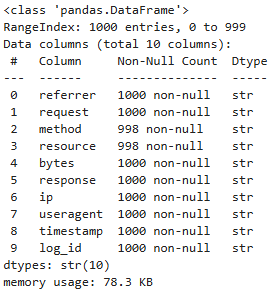
\includegraphics[width=0.5\textwidth]{Immagini/df_info_pandas.png}
      \caption{Output della funzione pd.DataFrame.info}
      \label{fig:df_info}
\end{figure}

Da una indagine più approfondita si constata che il server ha restituito response di tipo 400 (\emph{Bad Request}) e 408 (\emph{Request Timeout}), imputabili a cause di natura sia client-side, come richieste malformate o incomplete, sia server-side, come timeout dovuti a congestione o ritardi nella gestione della connessione, comportando quindi la mancata registrazione di alcuni campi essenziali come method e resource. Questa premessa ci permetterà una analisi più approfondita in seguito.

\section{Aggiunta al dataset di attacchi artificiali}

Al fine di testare la capacità di rilevamento del sistema, il dataset è stato integrato con dei record sintetici appositamente progettati per rappresentare minacce web esplicite. Tali istanze, pur mantenendo la coerenza strutturale con il traffico legittimo presente nel dataset, presentano anomalie semantiche riconducibili a pattern di attacco noti.

Di seguito si riporta un esempio di record configurato per simulare un attacco di tipo Cross-Site Scripting (XSS):



\begin{lstlisting}[language=json, caption={Esempio di log JSON con attacco XSS}, label={lst:xss_log}]
{
  "referrer": "http://search.lib.auth.gr/Search/<script>alert('XSS')</script>",
  "request": "search.lib.auth.gr:80 185.22.12.44 - - [01/Mar/2018:00:00:15 +0200] GET /Search?q=<script>alert('XSS')</script> HTTP/1.1 400 1200",
  "method": "GET",
  "resource": "/Search?q=<script>alert('XSS')</script>",
  "bytes": "1200",
  "response": "400",
  "ip": "185.22.12.44",
  "useragent": "Mozilla/5.0",
  "timestamp": "2018-02-28T22:00:15.000Z",
  "log_id": "attack_xss"
}
\end{lstlisting}

Per facilità di lettura, questi record sono stati catalogati con la voce \emph{attack} nel campo \emph{log\_id} in maniera tale da rendere più facile, in un successivo momento, l’estrazione degli stessi.

\section{Ingegneria delle feature}

Al fine di rendere il dataset interpretabile dall’algoritmo di Isolation Forest, quest’ultimo è stato sottoposto ad un processo di estrazione di nuove caratteristiche (\emph{features}). L’obiettivo è trasformare i log testuali in indicatori numerici e booleani che quantifichino anomalie strutturali, sintattiche e comportamentali nel traffico di rete.

Le feature prese in considerazione e riportate di seguito possono essere raggruppate sostanzialmente in tre macrocategorie: Analisi dimensionale, pattern matching e firme di attacco, analisi statistica e comportamentale


\begin{enumerate}
      \item Analisi dimensionale. \\
            Le anomalie nelle dimensioni indicano spesso tentativi di \emph{buffer overflow} o iniezioni di \emph{payload} estesi.

            \renewcommand{\labelenumii}{\theenumi.\arabic{enumii}}
            \begin{enumerate}
                  \item \texttt{resource\_len} (Lunghezza della risorsa):

                        Descrizione: Calcola il numero di caratteri che compongono la stringa della risorsa richiesta (\emph{URI}).

                        Razionale: Le richieste benigne tendono a raggrupparsi attorno a lunghezze standard \parencite{kruegel2003anomaly}. Poiché l'algoritmo Isolation Forest è progettato per identificare le anomalie isolando i campioni rari e dimensionalmente distanti (\emph{outlier}), fornire in input la lunghezza esatta della risorsa permette agli alberi di separare i \emph{payload} d'attacco con pochissimi split logici, aumentando l'efficienza computazionale e l'accuratezza del rilevamento.
                  \item \texttt{has\_suspicious\_request\_len} (Anomalia dimensionale della risorsa):

                        Descrizione: Applica il metodo statistico del Range Interquartilico (IQR) sulla lunghezza della risorsa. Assegna il valore 0 (normale) se la lunghezza rientra nell’intervallo
                        \begin{equation}
                              Q_1 - 1.5 \times \text{IQR} \le x \le Q_3 + 1.5 \times \text{IQR}
                        \end{equation}
                        e 1 (sospetto) in caso contrario.

                        Razionale: Fornisce al modello una classificazione pre-calcolata degli outlier unidimensionali, facilitando il partizionamento dei record palesemente anomali \parencite{kruegel2003anomaly}.
            \end{enumerate}
            % Fine sottolistap

      \item Pattern matching e firme di attacco (Analisi lessicale).\\
            Queste feature binarie (0/1) ricercano la presenza di sintassi associata a vettori di attacco noti o a strumenti di scansione automatizzata.

            \begin{enumerate}
                  \item \texttt{special\_char} (Conteggio dei caratteri speciali):

                        Descrizione: Conta le occorrenze di caratteri non alfanumerici (es. \texttt{<} \texttt{>} \texttt{'} \texttt{"} \texttt{\%} \texttt{;} \texttt{(} \texttt{)} \texttt{\{} \texttt{\}} \texttt{*} \texttt{+} \texttt{@}).

                        Razionale: Un'alta concentrazione di questi caratteri devia fortemente dalla baseline del traffico normale \parencite{kruegel2003anomaly}, fornendo all'Isolation Forest una metrica numerica netta per separare i payload malevoli.

                  \item \texttt{has\_traversal} (Rilevamento Path Traversal):

                        Descrizione: : Identifica la sequenza  \emph{../} nel corpo della richiesta.

                        Razionale: L’utilizzo della sequenza citata identifica un tentativo di risalita delle directory del server \parencite{owasp2021a01} \parencite{mitre_cwe22}.
                  \item \texttt{has\_sql\_keywords} (Rilevamento \emph{SQL Injection - SQLi}):

                        Descrizione: : Verifica la presenza di parole chiave tipiche del linguaggio SQL (\emph{union, select, insert, drop}) o tautologie (\emph{or 1=1, --, admin}).

                        Razionale: attacchi informatici come SQL Injection usano delle parole chiave che tentano di manipolare le query di backend del database \parencite{owasp2021a03}.

                  \item \texttt{has\_script\_tag} (Rilevamento \emph{Cross-Site Scripting - XSS}):

                        Descrizione: : Ricerca il tag \texttt{<script>} all’interno della richiesta.

                        Razionale: la ricerca mira ad identificare l’iniezione di codice eseguibile lato client, tipica degli attacchi XSS \parencite{owasp2021a03}.

                  \item \texttt{scanner\_agent} (Rilevamento \emph{User-Agent} malevoli):

                        Descrizione: Cerca stringhe associate a noti tool di vulnerability scanning o exploitation automatizzata (es. sqlmap, nikto, nmap, dirbuster, o l'uso base di curl).

                        Razionale: Gli strumenti di scanning automatici lasciano tracce estremamente evidenti, a meno che l’attaccante non compia sforzi deliberati per nasconderle. Ogni software che effettua richieste HTTP deve dichiararsi tramite l’header user-agent \parencite{nikto_useragent} \parencite{sqlmap_useragent} \parencite{nmap_useragent}.

                        L'efficacia della feature \emph{scanner\_agent} è supportata dalla natura stessa dei tool di \emph{vulnerability scanning}, i quali, nelle configurazioni predefinite, includono identificativi univoci all'interno dell'header \emph{HTTP User-Agent}. Tale comportamento è ampiamente documentato sia nelle specifiche tecniche degli strumenti stessi, sia nei set di regole dei principali Web Application Firewall che utilizzano queste “firme” per la chiusura immediata delle connessioni sospette.

                  \item \texttt{is\_known\_bot} (Identificazione di crawler e motori di ricerca tramite keyword):

                        Descrizione: Questa feature esegue una scansione del campo \emph{useragent} alla ricerca di stringhe identificative (\emph{keyword}) riconducibili a crawler benevoli e bot di indicizzazione (es. \emph{Googlebot, Bingbot, DotBot}).

                        Razionale: Durante le fasi preliminari di sperimentazione, è emerso che l'attività dei crawler generava un elevato numero di falsi positivi. Tali agenti automatizzati presentano profili di navigazione (frequenza di richiesta, esplorazione sistematica delle directory e parametri complessi) che l'Isolation Forest interpreta nativamente come anomalie. L'introduzione di questa feature permette al modello di pesare correttamente questo "rumore di fondo", distinguendo tra l'automazione finalizzata all'indicizzazione (benigna) e l'automazione finalizzata all'attacco (maligna).

            \end{enumerate}

      \item Analisi Statistica e Comportamentale.\\
            Queste metriche valutano il comportamento dell'utente e la risposta del server, fornendo un contesto più ampio rispetto alla singola riga di log.

            \renewcommand{\labelenumii}{\theenumi.\arabic{enumii}}
            \begin{enumerate}
                  \item \texttt{is\_error} (Codici di stato HTTP di errore):

                        Descrizione: Flag binario che indica se il server ha risposto con un codice di errore (status code $\geq$ 400)

                        Razionale: Gli attaccanti che effettuano brute-force o fuzzing, generano un'alta percentuale di risposte HTTP 400 (\emph{Bad Request}), 403 (\emph{Forbidden}) o 404 (\emph{Not Found}) \parencite{kruegel2003anomaly}.

                  \item \texttt{num\_params} (Complessità della Query String):

                        Descrizione: Conta il numero di parametri passati nella risorsa (contando il carattere =).

                        Razionale: Le pagine prese di mira per le iniezioni (SQLi, XSS) presentano spesso query string complesse per il passaggio dei payload \parencite{kruegel2003anomaly}. Più parametri sono presenti, maggiore è la probabilità che si tratti di una injection o tentativo di manipolazione.

                  \item \texttt{request\_per\_ip} (Frequenza di richiesta per host):

                        Descrizione: Calcola il numero totale di richieste effettuate da un singolo indirizzo IP rappresentando la densità di traffico generata da un singolo client.

                        Razionale: Valori anomali in questa metrica sono il sintomo primario di attacchi volumetrici \parencite{mitrebruteforce} \parencite{mitredos} \parencite{thottan2003anomaly}. Mentre le feature precedenti analizzano il contenuto, questa analizza quante richieste vengono fatte da un singolo indirizzo IP, rendendolo di fatto un parametro chiave per l’algoritmo nel distinguere utenti umani da script automatici.

                  \item \texttt{request\_entropy} (Entropia di Shannon della richiesta):

                        Descrizione: Calcola l'entropia della stringa di richiesta utilizzando la formula:
                        \begin{equation}
                              H(X) = - \sum_{i=1}^{n} p(x_i) \log_{2} p(x_i)
                        \end{equation}
                        Razionale: L'entropia misura il grado di "disordine" o casualità della stringa. Payload offuscati (es. codifica Base64), shellcode o stringhe generate algoritmicamente (DGA) presentano un'entropia significativamente maggiore rispetto alle normali URL legittime dove sono presenti parole di senso compiuto e strutture ripetitive \parencite{lyda2007using}

                        Nota Metodologica: Si osserva che nel dataset utilizzato per il presente caso studio, i campi testuali sono stati preventivamente sottoposti a un processo di hashing per ragioni di anonimizzazione e privacy. Poiché le funzioni di hash sono progettate per massimizzare la diffusione e produrre stringhe ad alta entropia indipendentemente dall'input originale, il valore di \texttt{request\_entropy} risulta uniformemente elevato per l'intero dataset. Pertanto, sebbene tale feature sia stata inclusa per completezza metodologica e per dimostrarne il valore predittivo in scenari di monitoraggio in chiaro (dove l'offuscamento malevolo si distingue nettamente dal testo naturale), nel contesto specifico di questo esperimento il suo apporto alla capacità discriminante dell'Isolation Forest è mitigato dalla natura crittografica dei dati sorgente.

                  \item \texttt{bytes\_ratio} (Rapporto di trasmferimento dati):

                        Descrizione: Calcola il rapporto tra i byte trasferiti in una specifica transazione e la media storica dei byte trasferiti per quella medesima risorsa.

                        Razionale: Mentre nel traffico ordinario la dimensione della risposta per una specifica risorsa URI tende a essere costante (bassa varianza), deviazioni significative nel volume di byte trasferiti indicano potenziali anomalie post-compromissione. Come evidenziato dal framework MITRE ATTACK nella tecnica T1020 (\emph{Automated Exfiltration}) \parencite{mitreT1020a}, il monitoraggio del volume cumulativo di dati permette di rilevare l'estrazione di informazioni sensibili tramite SQL Injection o accessi non autorizzati, rendendo tale rapporto un input critico per l'algoritmo di isolamento.



            \end{enumerate}

\end{enumerate}

\section{Applicazione dell'algoritmo}

L’algoritmo di Isolation Forest opera attraverso partizioni casuali dello spazio delle feature \parencite{liu2008isolation}; per questo motivo, il dataset è stato ridotto alle sole componenti numeriche e booleane derivate.

Sebbene l'algoritmo sia intrinsecamente invariante alla scala, è stato scelto di integrare un MinMaxScaler all'interno della pipeline di addestramento.

Nota Metodologica: L'uso della normalizzazione in questo caso studio non è dettato dai vincoli del modello di isolamento, ma dalla necessità di stabilizzare il processo di \emph{Hyperparameter Tuning}. Scalando le feature in un range $[0, 1]$, si garantisce che durante la fase di \emph{Grid Search} il calcolo delle metriche di scoring avvenga su una distribuzione controllata, facilitando la convergenza verso i parametri ottimali.

Per evitare una scelta arbitraria dei parametri (come la contamination o il numero di alberi), è stata implementata una ricerca sistematica tramite \emph{GridSearchCV}. Questo approccio trasforma un modello tipicamente non supervisionato in un sistema "guidato" dai dati reali (nel caso studio, gli attacchi inseriti manualmente).

\begin{itemize}
      \item Scoring Strategy: È stata scelta la \emph{recall\_macro} come metrica di riferimento (\texttt{refit='rec'}). In un contesto come quello del presente caso studio, è prioritario massimizzare il richiamo (\emph{Recall}), ovvero la capacità del sistema di non farsi sfuggire i veri attacchi, anche a costo di accettare un numero leggermente superiore di falsi positivi.
      \item Risultati dell'Ottimizzazione e Parametri ottimali:\\
            La configurazione ottimale identificata ha prodotto un Recall di $\sim$0.79 con i valori di \texttt{contamination} e \texttt{n\_estimators} impostati rispettivamente a 0.01 e 1000.
\end{itemize}

Un passaggio tecnico fondamentale riguarda la mappatura delle classi per la compatibilità con la libreria Scikit-Learn. Poichè l'Isolation Forest restituisce -1 per le anomalie e 1 per il traffico normale, le etichette del Ground Truth sono state allineate in tal senso.

\begin{lstlisting}[style=MatlabStyle, caption={}, label={lst:prova}]
    df['is_attack_real'] = df['log_id'].str.contains('attack').astype(int)
    df.loc[df['is_attack_real'] == 1, 'is_attack_real'] = -1
    df.loc[df['is_attack_real'] == 0, 'is_attack_real'] = 1
\end{lstlisting}

Questo allineamento permette alle funzioni di scoring della Grid Search di interpretare correttamente le anomalie come la classe di interesse da rilevare.

\section{Interpretazione dei risultati}

L'algoritmo Isolation Forest non restituisce un verdetto binario deterministico, bensì un valore di "anomalia" continuo. Mentre i punteggi negativi più profondi identificano record con feature multiple "fuori scala" (ovvero campioni che richiedono pochissimi partizionamenti per essere isolati), i punteggi prossimi allo zero rappresentano una zona di incertezza statistica dove solitamente ricadono i falsi positivi.

Si riporta di seguito un primo snippet di codice e la relativa tabella per verificare come l'algoritmo abbia classificato gli attacchi inseriti artificialmente nel dataset per testare la sensibilità del modello:

\begin{lstlisting}[style=MatlabStyle, caption={Verifica classificazione attacchi artificiali}, label={lst:interpretazione}]
df[df['log_id'].str.contains('attack')][['log_id', 'anomaly_score', 'scores']]
\end{lstlisting}

\begin{table}[H]
      \centering
      \begin{tabular}{|c|c|c|c|}
            \hline
            Index & log\_id           & anomaly\_score & scores    \\
            \hline
            1000  & attack\_xss       & -1             & -0.065746 \\
            1001  & attack\_sql       & -1             & -0.110561 \\
            1002  & attack\_traversal & -1             & -0.125805 \\
            1003  & attack\_scanner   & -1             & -0.138416 \\
            \hline
      \end{tabular}
      \caption{Scores per gli attacchi artificiali}
\end{table}


Come si evince dai risultati, tutti gli attacchi iniettati sono stati correttamente identificati come anomalie (\texttt{anomaly\_score = -1}), con punteggi di isolamento significativamente bassi, confermando l'efficacia delle feature estratte nel caratterizzare pattern malevoli noti.

Per convalidare il caso studio, si è proceduto al calcolo della matrice di confusione e del relativo \emph{classification report}. Questi strumenti sono essenziali per misurare la capacità del modello di distinguere tra traffico lecito e tentativi di intrusione.

\begin{figure}[H]
      \centering
      \includegraphics[width=\textwidth]{Immagini/Matrice\_di\_confusione.png}
      \caption{Matrice di confusione}
      \label{fig:mdc}
\end{figure}


\begin{lstlisting}[style=MatlabStyle, caption={Generazione del Classification Report}, label={lst:prova}]
from sklearn.metrics import classification_report
print(classification_report(df['is_attack_real'], df['is_attack_predicted']))
\end{lstlisting}

\begin{table}[H]
      \centering
      \begin{tabular}{|c|c|c|c|c|}
            \hline
            \dots        & precision & recall & f1-scores & support \\
            \hline
            0            & 1.00      & 0.99   & 1.00      & 998     \\
            1            & 0.36      & 1.00   & 0.53      & 4       \\

            accuracy     & -         & -      & 0.99      & 1002    \\
            macro avg    & 0.68      & 1.00   & 0.76      & 1002    \\
            weighted avg & 1.00      & 0.99   & 0.99      & 1002    \\

            \hline
      \end{tabular}
      \caption{Classification report}
\end{table}

L'analisi del report evidenzia una \textbf{Recall} del 100\% sulla classe 1 (attacchi), indicando che il modello non ha generato falsi negativi. Tuttavia, la \textbf{Precision} si attesta allo 0.36; questo valore, pur sembrando basso in un contesto di classificazione standard, è tipico dei sistemi di \emph{Anomaly Detection}. Come sottolineato da Sommer e Paxson \parencite{sommer2010outside}, nei sistemi di \emph{intrusion detection} basati su anomalie l’elevata incidenza di falsi positivi rappresenta uno dei principali limiti all’adozione in ambito operativo, in quanto attività lecite ma atipiche possono facilmente essere classificate come sospette.


Oltre agli attacchi artificiali, il modello ha catalogato come anomalie altri record presenti nel traffico originale. Di seguito vengono riportati i campioni con il punteggio di isolamento più basso:

\begin{lstlisting}[style=MatlabStyle, caption={Estrazione delle top anomalie}, label={lst:top_anomalies}]
top_anomalies = df[df['anomaly_score']==-1][['request','scores']].sort_values(by='scores')
\end{lstlisting}

\begin{table}[H]
      \centering

      \vspace{1mm}
      \resizebox{\textwidth}{!}{%
            \begin{tabular}{|c|p{20cm}|}
                  \hline
                  \textbf{Index} & \textbf{Request Log Entry}                                                                                                                                  \\ \hline
                  1003           & {\ttfamily search.lib.auth.gr:80 203.0.113.45 - - [01/Mar/2018:00:00:30 +0200] GET /wp-admin/install.php HTTP/1.1 404 250 - sqlmap/1.7}                     \\ \hline
                  1002           & {\ttfamily search.lib.auth.gr:80 91.200.12.77 - - [01/Mar/2018:00:00:25 +0200] GET /../../../../etc/passwd HTTP/1.1 403 300 - curl/7.58.0}                  \\ \hline
                  1001           & {\ttfamily search.lib.auth.gr:80 45.77.88.12 - - [01/Mar/2018:00:00:20 +0200] GET /login?user=admin' OR 1=1-- HTTP/1.1 500 800 http://evil.com Mozilla/5.0} \\ \hline
                  1000           & {\ttfamily search.lib.auth.gr:80 185.22.12.44 - - [01/Mar/2018:00:00:15 +0200] GET /Search?q=<script>alert('XSS')</script> HTTP/1.1 400 1200 ...}           \\ \hline
                  918            & {\ttfamily search.lib.auth.gr:80 176.92.34367 - - [01/Mar/2018:00:07:56 +0200] GET /Cover/Show?author=Winstanley... HTTP/1.1 200 677}                       \\ \hline
                  826            & {\ttfamily search.lib.auth.gr:80 176.92.34367 - - [01/Mar/2018:00:07:34 +0200] GET /Cover/Show?author=... HTTP/1.1 200 678}                                 \\ \hline
                  629            & {\ttfamily search.lib.auth.gr:80 155.207.36594 - - [01/Mar/2018:00:05:46 +0200] GET /Cover/Show?author=... HTTP/1.1 200 677}                                \\ \hline
                  497            & {\ttfamily search.lib.auth.gr:80 176.92.58901 - - [01/Mar/2018:00:05:08 +0200] GET / HTTP/1.1 200 4709 - Mozilla/5.0}                                       \\ \hline
                  429            & {\ttfamily search.lib.auth.gr:80 66.249.58337 - - [01/Mar/2018:00:04:25 +0200] GET /themes/jquerymobile/... HTTP/1.1 200 32415}                             \\ \hline
                  327            & {\ttfamily search.lib.auth.gr:80 85.74.35922 - - [01/Mar/2018:00:03:05 +0200] GET /themes/bootstrap3/... HTTP/1.1 200 65714}                                \\ \hline
                  59             & {\ttfamily search.lib.auth.gr:80 141.237.44390 - - [01/Mar/2018:00:00:19 +0200] GET /themes/bootstrap3/... HTTP/1.1 200 65714}                              \\ \hline
            \end{tabular}
      }
      \caption{Anomalie per punteggio di \emph{scores}}
\end{table}


Da un'analisi approfondita, emerge che tali richieste non appartengono al "rumore di fondo" generato dai crawler (correttamente filtrati dalla feature \\ \texttt{is\_known\_bot}), ma presentano valori di \texttt{resource\_len} e \texttt{bytes\_num} estremamente distanti dalla media. Ad esempio, le richieste ai temi grafici (Index 327, 59) o i file CSS/JS molto pesanti vengono isolati per la loro mole di dati. Nonostante la loro natura anomala dal punto di vista statistico, essi possono essere classificati come falsi positivi in ambito di sicurezza, rappresentando traffico lecito ma strutturalmente pesante.

\section{Applicazione dell'algoritmo all'intero dataset}

Nelle sezioni precedenti, al fine di condurre una fase esplorativa e calibrare i parametri dell’algoritmo, l’analisi è stata inizialmente limitata ai primi 1000 record del dataset.

Per verificare la tenuta del modello in uno scenario più realistico, l’algoritmo è stato successivamente applicato all’intero dataset. Questa seconda valutazione ha evidenziato uno dei principali limiti dell’Isolation Forest in contesti fortemente sbilanciati: i quattro attacchi inseriti manualmente non emergono più con sufficiente evidenza quando vengono immersi in un corpus di circa quattro milioni di record. In tale scenario, il modello attribuisce l’etichetta di anomalia a un numero molto elevato di osservazioni, circa 100.000, ma riflettono soprattutto traffico legittimo statisticamente atipico.

\begin{figure}[H]
      \centering
      \includegraphics[width=\textwidth]{Immagini/Matrice\_di\_confusione\_all.png}
      \caption{Matrice di confusione applicata all'intero dataset}
      \label{fig:mdcall}
\end{figure}

Dopo una più approfondita operazione di clustering ricavato dalla seguente query:

\begin{lstlisting}[style=MatlabStyle, caption={}, label={lst:topanomalies}]
    top_anomalies = df[df["anomaly_score"] == -1].sort_values(by='scores')
    top_anomalies_melted = top_anomalies.melt(
    id_vars='log_id',
    var_name='categories',
    value_vars=features_boolean,
    value_name='value')

active = top_anomalies_melted[top_anomalies_melted['value'] == 1]
combos = active.groupby('log_id')['categories'].agg(lambda x: ", ".join(tuple(sorted(x)))).reset_index(name='tuple')
\end{lstlisting}

Si estrapola la seguente tabella:

\begin{table}[H]
      \centering
      \begin{tabular}{|l|r|}
            \hline
            \textbf{Combinazione di Feature}                                         & \textbf{Frequenza} \\
            \hline
            is\_known\_bot, special\_chars                                           & 86.654             \\
            has\_suspicious\_request\_len                                            & 4.033              \\
            has\_suspicious\_request\_len, is\_known\_bot, special\_chars            & 3.011              \\
            has\_suspicious\_request\_len, is\_known\_bot                            & 2.879              \\
            is\_known\_bot                                                           & 2.556              \\
            has\_suspicious\_request\_len, is\_error                                 & 1.340              \\
            has\_sql\_keywords, has\_suspicious\_request\_len, is\_error             & 164                \\
            has\_suspicious\_request\_len, is\_error, is\_known\_bot                 & 131                \\
            is\_error, is\_known\_bot, special\_chars                                & 86                 \\
            has\_suspicious\_request\_len, special\_chars                            & 68                 \\
            is\_error, is\_known\_bot                                                & 34                 \\
            has\_sql\_keywords, has\_suspicious\_request\_len                        & 15                 \\
            is\_error                                                                & 4                  \\
            has\_suspicious\_request\_len, is\_error, is\_known\_bot, special\_chars & 1                  \\
            \hline
      \end{tabular}
      \caption{Report di classificazione delle occorrenze per combinazione di feature.}
\end{table}

L’analisi delle combinazioni di feature mostra che molte delle osservazioni segnalate come anomale condividono attributi ricorrenti come \emph{is\_known\_bot}, \emph{special\_chars} e \emph{has\_suspicious\_request\_len}. Questo suggerisce che il modello non sta isolando esclusivamente gli attacchi, ma intercetta anche pattern statistici frequenti nel traffico legittimo, in particolare richieste generate da crawler o risorse di dimensione insolita. Di conseguenza, l’anomalia rilevata dal modello non coincide sempre con un evento di sicurezza, ma spesso con una deviazione rispetto alla normalità statistica del dataset

Per visualizzare l’effetto del forte sbilanciamento del dataset, si riporta un grafico boxplot degli anomaly score rispetto alla posizione del record nel dataframe sia per il caso di un dataset limitato, sia per il caso del dataset completo.

\begin{figure}[H]
      \centering
      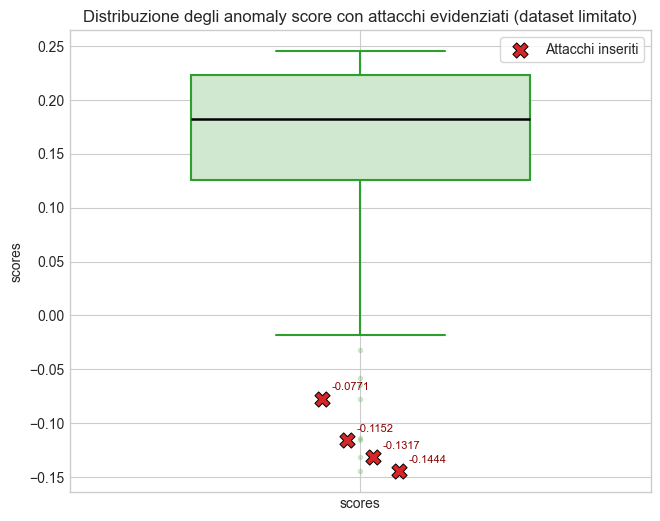
\includegraphics[width=\textwidth]{Immagini/boxplotlimited.png}
      \caption{Boxplot distribuzione anomalie (Dataset limitato ai primi 1000 record)}
      \label{fig:boxplotlimit}
\end{figure}

Per il dataset limitato, il boxplot mostra che i 4 attacchi cadono chiaramente nella zona di coda e vengono facilmente separati dalla distribuzione principale.

\begin{figure}[H]
      \centering
      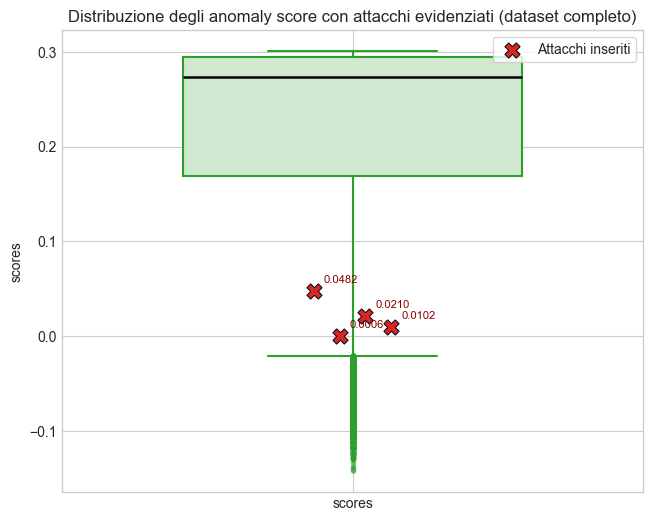
\includegraphics[width=\textwidth]{Immagini/boxplotall.png}
      \caption{Boxplot distribuzione anomalie (Dataset intero)}
      \label{fig:boxplotall}
\end{figure}

Per il dataset completo, la distribuzione degli score mostra uno sbilanciamento più accentuato e il segnale dei quattro attacchi perde forza discriminante, poichè la soglia di anomalia non li isola più in modo affidabile rispetto ai valori anomali dell'intero dataset.

\chapter{Conclusioni}

\section{Sintesi del caso studio}

Il presente lavoro di tesi ha avuto come obiettivo la progettazione, l’implementazione e la valutazione di un sistema di \emph{Anomaly Detection} basato sull’algoritmo Isolation Forest, applicato all’analisi di log HTTP provenienti da un contesto reale. L’intero percorso di sviluppo è stato impostato con una finalità duplice: da un lato, verificare la fattibilità di un approccio automatico al rilevamento di comportamenti anomali nei log web; dall’altro, valutare in modo critico fino a che punto un modello non supervisionato possa essere utile in uno scenario applicativo concreto, caratterizzato da un forte squilibrio tra traffico lecito e richieste potenzialmente malevole.

Il punto di partenza dell’elaborato risiede nella constatazione che i sistemi di difesa tradizionali, fondati su regole statiche, firme note o blacklist manuali, mostrano limiti significativi nel fronteggiare la crescente dinamicità delle minacce informatiche e la variabilità del traffico web moderno. In un contesto di questo tipo, l’adozione di tecniche di Machine Learning rappresenta un’alternativa interessante, poiché consente di intercettare deviazioni dal comportamento atteso anche in assenza di una conoscenza preventiva di tutte le tipologie di attacco. Tale impostazione è particolarmente rilevante nei sistemi di analisi dei log, dove l’obiettivo non è soltanto individuare eventi noti, ma anche evidenziare pattern rari, sospetti o non immediatamente riconducibili a regole predefinite.

L’attività svolta si è concentrata sulla costruzione di un dataset derivato da log HTTP, sottoposto a un processo di pre-processing e di \emph{feature engineering} finalizzato a trasformare l’informazione testuale in variabili numeriche e booleane interpretabili dall’algoritmo. Le feature selezionate sono state progettate con un criterio orientato alla sicurezza applicativa: alcune descrivono caratteristiche dimensionali delle richieste, altre cercano pattern sintattici riconducibili a vettori d’attacco noti, altre ancora cercano di modellare aspetti comportamentali del traffico. Questo passaggio metodologico è stato centrale, perché nel caso di log web la qualità delle feature incide in modo determinante sulla capacità del modello di separare eventi normali, anomalie statistiche e vere anomalie di sicurezza.

L’algoritmo Isolation Forest è stato applicato dapprima a un sottoinsieme ridotto del dataset, così da consentire una prima fase esplorativa e una calibrazione ragionata dei parametri. In questo scenario limitato, il modello ha mostrato una discreta capacità di individuare gli attacchi inseriti manualmente, confermando che la combinazione tra feature engineering e anomaly scoring può produrre risultati utili quando il problema è ben circoscritto e il segnale anomalo è ancora distinguibile dal rumore di fondo. Questa fase ha quindi avuto un valore soprattutto dimostrativo e metodologico, oltre che sperimentale.

Tuttavia, l’estensione dell’analisi all’intero dataset ha mostrato con chiarezza i limiti dell’approccio adottato. Quando il modello viene applicato a un corpus di dimensioni molto elevate, con milioni di record e una quota di anomalie estremamente ridotta, la capacità discriminante dell’Isolation Forest si indebolisce sensibilmente. In particolare, i quattro attacchi inseriti manualmente non riescono più a emergere con affidabilità sufficiente rispetto alla massa dei log leciti, e il modello finisce per segnalare soprattutto osservazioni statisticamente atipiche ma non necessariamente malevole. Questo comportamento evidenzia un aspetto cruciale: in un contesto molto sbilanciato, il confine tra anomalia statistica e anomalia di sicurezza tende a sfumare, e il modello può privilegiare la forma del dato rispetto al suo significato operativo.

Un ulteriore elemento emerso dall’analisi riguarda il rapporto tra richiamo e precisione. L’Isolation Forest, soprattutto in configurazioni orientate alla massima sensibilità, tende a intercettare un numero elevato di outlier, ma questo si accompagna inevitabilmente a un aumento dei falsi positivi. Nel dominio della cybersecurity ciò non rappresenta soltanto un dettaglio tecnico, ma una questione sostanziale: un sistema che produce troppe segnalazioni non rilevanti rischia di ridurre la fiducia degli analisti e di abbassare l’efficacia operativa complessiva della soluzione. Di conseguenza, un buon modello di anomaly detection non deve limitarsi a “vedere tanto”, ma deve anche saper discriminare in modo sufficientemente fine ciò che merita realmente attenzione.

In questo senso, il lavoro conferma che l’Isolation Forest è uno strumento molto utile come base esplorativa, soprattutto quando si dispone di pochi esempi etichettati e si desidera ottenere una prima fotografia del comportamento del traffico. Il suo principale vantaggio è la scalabilità concettuale e computazionale; il suo principale limite, invece, emerge proprio quando il dataset cresce molto e il rumore supera il segnale. In tali condizioni, il modello tende a identificare soprattutto deviazioni statistiche generiche, mentre gli attacchi reali, se troppo pochi e troppo immersi nella distribuzione complessiva, possono perdere visibilità.

La lettura congiunta della matrice di confusione, del classification report e delle combinazioni di feature più frequenti tra le anomalie individuate porta a una conclusione chiara: il sistema non va interpretato come un sostituto dei meccanismi di difesa tradizionali, ma come uno strumento complementare di supporto all’analisi. In un contesto operativo reale, un approccio di questo tipo dovrebbe essere integrato con ulteriori filtri, controlli a valle, regole di priorizzazione o componenti supervisionate, così da ridurre l’impatto dei falsi positivi e aumentare la probabilità di intercettare gli eventi davvero critici.

\section{Considerazioni finali}

Dal punto di vista metodologico, l’esperienza svolta mette in evidenza alcuni elementi di valore generale. In primo luogo, mostra che l’analisi dei log HTTP può fornire informazioni estremamente utili non solo per la diagnostica e il monitoraggio, ma anche per attività di sicurezza orientate al rilevamento automatico di pattern anomali. In secondo luogo, evidenzia che il successo di un progetto di anomaly detection dipende in larga misura dalla qualità della rappresentazione dei dati: scegliere le feature giuste, definire correttamente le etichette e interpretare in modo critico gli score prodotti dal modello sono passaggi decisivi quanto la scelta dell’algoritmo stesso.

Il caso studio ha inoltre mostrato che, nei problemi di sicurezza applicata, le metriche vanno lette con attenzione e mai isolate dal contesto. Un risultato apparentemente alto in termini di accuracy può risultare fuorviante se il dataset è fortemente sbilanciato; allo stesso modo, una buona recall sugli attacchi non garantisce automaticamente l’utilizzabilità del sistema, se la precisione resta troppo bassa e il numero di falsi positivi diventa eccessivo. In altre parole, non basta che il modello sia “tecnicamente corretto”: deve essere anche coerente con l’obiettivo operativo per cui viene impiegato.

Un altro aspetto importante riguarda il ruolo della conoscenza di dominio. Nel caso dei log HTTP, l’interpretazione dei risultati beneficia fortemente della comprensione del contesto applicativo: richieste lunghe, crawler, strumenti automatici di scansione e pattern sintattici sospetti non hanno tutti lo stesso significato. Alcuni rappresentano segnali potenzialmente malevoli, altri sono semplicemente caratteristiche atipiche di traffico legittimo. La capacità di distinguere questi casi richiede non solo un modello, ma anche un’analisi critica umana e, idealmente, un ciclo di feedback continuo tra sistema automatico e validazione esperta.

Sotto il profilo dei risultati, il lavoro conferma quindi un punto fondamentale: l’Isolation Forest è efficace come **strumento esplorativo**, ma non è sufficiente, da solo, a risolvere il problema del rilevamento automatico di anomalie in contesti molto grandi e rumorosi. Nel sottoinsieme ridotto del dataset il modello riesce a evidenziare gli attacchi inseriti manualmente con una certa chiarezza; sull’intero corpus, invece, la sua capacità di generalizzazione si riduce sensibilmente, e gli attacchi finiscono per essere assorbiti dalla massa dei log normali e dalle anomalie statistiche non rilevanti dal punto di vista della sicurezza. Questo non invalida il metodo, ma ne delimita con precisione il campo di applicazione.

In conclusione, il lavoro svolto rappresenta un passo concreto verso sistemi di analisi dei log più intelligenti e adattivi, ma evidenzia anche che l’automazione del rilevamento non può prescindere da un’integrazione con altre forme di controllo. Le possibili evoluzioni future includono l’uso di modelli ibridi, l’introduzione di meccanismi supervisionati o semi-supervisionati, l’affinamento delle feature, l’ottimizzazione della soglia decisionale e l’adozione di strategie di post-processing basate sul feedback dell’analista. L’obiettivo non dovrebbe essere soltanto ridurre il numero di errori, ma costruire un sistema capace di trasformare i segnali grezzi del traffico web in informazioni davvero utili, affidabili e azionabili.

\chapter*{Ringraziamenti}
\addcontentsline{toc}{chapter}{Ringraziamenti}

A conclusione di questo elaborato desideravo fare menzione di tutti coloro i quali che in questi anni hanno contribuito (direttamente ed indirettamente) al compimento del mio iter accademico.

Desidero innanzitutto esprimere la mia più sincera gratitudine al Prof. Bellone, per la disponibilità, la guida ed i preziosi suggerimenti che hanno reso possibile la realizzazione di questo lavoro.

Un ringraziamento particolare ai colleghi di lavoro Sergio e Luca che mi hanno supportato (e sopportato) in questo periodo trascorso tra codice, script e stress sia lavorativi che accademici.

Un pensiero va agli amici (c.d. "Disagiati") di una vita che sono riusciti ad alleggerirmi la testa nei momenti dove ne avevo più bisogno.

Un ringraziamento particolare va a Giulia, compagna da un tempo che ormai sembra una vita. Senza di lei che è stata un supporto costante in tutto e per tutto, forse non avrei concluso questo iter.

Ed infine un grazie va a mio padre. Quasi trenta anni fa mi mettevi davanti ad un pc per la prima volta e mi dicevi:

\guillemetleft \emph{...Per far partire \emph{Seawolf} devi aprire la shell e chiamare il .exe} \guillemetright

Forse non sapevi che con quel piccolo gesto avresti condannato per sempre un ragazzo alla passione per la navigazione e l'informatica.
Grazie di cuore.

\chapter*{Sinossi}

\section*{Obbiettivi e contesto}
La presente tesi pone come obiettivo centrale la progettazione e realizzazione di un sistema prototipale che, sfruttando algoritmi di machine learning, sia in grado di analizzare automaticamente i log generati dai web server e rilevare eventuali anomalie o minacce.

La crescente evoluzione del panorama informatico ha reso sempre più urgente la necessità di individuare tempestivamente le minacce che possono originarsi dalle infrastrutture web ed i metodi convenzionali, basati su regole statiche o sull’impiego di blacklist, manifestano significative limitazioni soprattutto in termini di scalabilità e adattabilità. La natura dinamica delle minacce informatiche richiede soluzioni che sappiano evolversi e rispondere in modo efficace ai cambiamenti continui del contesto tecnologico.

Questo approccio mira a rispondere alla crescente necessità di individuazione tempestiva di tutto lo spettro delle possibili minacce offrendo un sistema più veloce e non supervisionato.

Dopo alcuni brevi cenni storici e metodologici sulla nascita, l'evoluzione ed il contesto inerenti il protocoloo HTTP ed analogamente ai concetti di Machine Learning e nel dettaglio dell'algoritmo di Isolation Forest, utili a fornire un quadro più chiaro sul contesto analizzato, si passa alla costruzione della logica dello script (questo visonabile nella repository GitHub al seguente link: \href{https://github.com/bellonemauro/http\_log\_analysis}{\emph{github.com/bellonemauro/http\_log\_analysis}})

\section*{Metodologia}

Il caso di studio si basa sull'analisi di un dataset di log HTTP reali sottoposti ad un \emph{pre-processing} per renderli idonei all'elaborazione automatizzata ed integrati con record artificiali volti a simulare delle anomalie derivante da tentativi di attacco informatico. L'algoritmo scelto è Isolation Forest, una tecnica di anomaly detection non supervisionata particolarmente efficiente per identificare osservazioni rare in grandi volumi di dati, grazie alla sua capacità di isolare i punti anomali tramite partizioni casuali dello spazio delle feature, riducendo l'impatto della \emph{curse of dimensionality}.


Il processo di implementazione ha previsto una fase di \emph{}{Feature Engineering}, ovvero la trasformazione dei log testuali in indicatori numerici e booleani basati su analisi dimensionale, \emph{pattern matching} (firme di attacco come \emph{SQLi} o \emph{XSS}) e analisi comportamentale; ed una fase di ottimizzazione che comprende l’utilizzo di \emph{GridSearchCV} per calibrare i parametri del modello (contamination e numero di alberi) in maniera automatica senza ricadere nella scelta arbitraria degli stessi, privilegiando la metrica \emph{recall} per minimizzare i falsi negativi e massimizzare l'identificazione degli attacchi ed infine l'addestramento del modello con relativi risultati, applicati sia ad un dataset limitato, sia all'intero log web.

\section*{Risultati e conclusioni}

L’esperimento ha dimostrato che, lavorando con un dataset limitato e circoscritto, il modello di Isolation Forest è efficace nell’identificare gli attacchi inseriti artificialmente, distinguendoli facilmente dal traffico normale.

Tuttavia, nel momento in cui l’algoritmo viene applicato all’intero dataset, che risulta un fortissimo sbilanciamento tra traffico lecito e minacce reali, le prestazioni diminuiscono drasticamente facendo si che l’algoritmo identifichi come anomalie attività lecite ma statisticamente atipiche, aumentando significativamente il numero dei falsi positivi ed ignorando quindi i record taggati in precedenza come “attacchi reali”.

In conclusione, la tesi evidenzia che l’Isolation Forest rappresenta un ottimo strumento esplorativo, ma da solo non può sostituire i meccanismi di difesa tradizionali. L’efficacia operativa in contesti reali richiede un approccio combinato di analisi automatizzata con filtri aggiuntivi, controlli supervisionati ed una costante validazione e ricerca umana per distinguere tra anomalie statistiche e reali minacce alla sicurezza.

\printbibliography

\end{document}